%==============================================================================
% Šablona prezentace/Presentation template
% Autoři / Authors: Zdeněk Vašíček, Aleš Smrčka, Jaroslav Dytrych, Jana Stopková, Kristýna Zaklová, Adam Herout
% Kontakt pro dotazy a připomínky: sablona@fit.vutbr.cz
% Contact for questions and comments: sablona@fit.vutbr.cz
%==============================================================================

%\documentclass[slovak]{fitthesispresn}
% Je-li prezentace v anglickém jazyce, je zapotřebí u třídy použít parametr english následovně (ev. zakomentovat předcházející řádek a odkomentovat následující): / If presentation is in English, it is necessary to use parameter english as follows (or comment the previous line and uncomment the following one):
\documentclass[english]{fitthesispresn}

% Nastavení informací pro úvodní stránku / Setting information for the title page
%---------------------------------------------------------------------------
\projectinfo{
  date={11.06.2024}, % Datum - je vhodné vepsat datum obhajoby (natvrdo), ne datum kompilace slajdů / Date - it is advisable to write the date of the defense (hard), not the date of the slide compilation        
  title={Blockchain Resistant\\to Quantum Attack}, % Název prezentace / Presentation title (The whole title of the presented work suitably divided into lines that are optically balanced)
  title.footer={Blockchain Resistant to Quantum Attack}, % Název prezentace - text zobrazovaný vedle čísla slajdu / Presentation title - displayed next to the slide number (The full title of the presented work, it may be suitably abbreviated to fit the footer)
  author.name={Michal},  % Jméno autora / Author name
  author.surname={Ľaš}, % Příjmení autora / Author surname
  author.title.first={}, % Tituly před jménem autora (jsou-li jaké) / Author's titles before the name (if there are any)
  supervisor.name={Kamil}, % Jméno vedoucího / Supervisor name
  supervisor.surname={Malinka}, % Příjmení vedoucího / Supervisor surname
  supervisor.title.first={Mgr.}, % Tituly před jménem / Supervisor's titles before the name
  supervisor.title.last={Ph.D.} % Tituly za jménem / Supervisor's titles after the name
}

% Struktura prezentace / Presentation structure
%---------------------------------------------------------------------------

\begin{document}
    \frame[plain]{\titlepage} % Úvodní stránka / Title page
    \ifczech
        %%%%%%%%                        01 - Motivace                       %%%%%%%%
%---------------------------------------------------------------------------
% Při prezentování nejvíc záleží na začátku. 
% Pro získání pozornosti na začátku veřejné řeči se doporučuje: říct nějakou statistiku; položit otázku (u státnic spíše řečnickou).



% <<<<<<<<<<<<<<<<<<<<<<<<<<<<<<<<<<<<<<<<<<<<<<<<< %
% TODO: otázka/štatistika

% Tips:
% 1. Novinky o kvantových počítačoch neajký pekný údaj. Nové kvantové PC, aký je ich výkon? Aké sú plány a vývoj?
% 2. "Bitcoin je momentálne celkom drahý. Cena okolo ... . Uvidíme či mu to vydrží aj po príchode kvantových počítačov."
% 3. Vyšli už nové štandardy od NIST? Aký je stav?

% Matoušek nemá moc rád bezpečnosť :) možno taktiež hodiť poznámku k tomu, že vývojari kvantových počítačov už 10 rokov hovoria, že budú moť dostatnočne výkonný počítač na prelomenie RSA.
% <<<<<<<<<<<<<<<<<<<<<<<<<<<<<<<<<<<<<<<<<<<<<<<<< %


%---------------------------------------------------------------------------

% - Uveďte posluchače do tématu své práce.
% - Řekněte něco málo o stavu před zahájením práce a jaké byly důvody pro její vypracování.
% - Nejlepší je vysvětlit motivaci pomocí schématu. Pokud musíte použít odrážky, tak super-stručné, abyste je nečetli, ale ony pouze tvořily kostru sdělení.

% Z této části prezentace musí posluchači dostat stručné a výstižné odpovědi na otázky:
%  A) Proč děláte, co děláte? K čemu je to dobré?
%  B) Co je cílem práce? Co má být výsledkem?

% Odolejte pokušení říkat banality a všeobecně známé informace.
% "Žijeme v době rozvoje mobilní výpočetní techniky, kdy každý má v kapse mobil" - je dokonale prázdné a hloupé sdělení, nic takového neříkejte, fakt to nikoho nezajímá.


% <<<<<<<<<<<<<<<<<<<<<<<<<<<<<<<<<<<<<<<<<<<<<<<<< %
% 1. Nejaký pekný obrázok: blockchain + kvantový počítač + hrozba
% 2. Prečo?: Kvantové počítače predstavujú nové hrozby pre kryptografiu na ktorej je technológia blockchain kriticky závislá. Preto je doležité adaptovať blockchain na nové hrozby ktoré kvantové počítače predstavujú.
% 3. Cieľ: Cieľom je teda identifikovať hrozby pre blockchainy, teda analyzovať zraniteľné časti blockchainu voči schopnostiam kvantových počítačov. Analyzovať vhodné PQ algoritmy pre blockchain a porovnať výkonnosť PQ algoritmu a súčasných v blockchaine (pripadne porovnať samotné blockchainy)
% - ciele možno napísať v odrážkach na ďalší slide, nech majú samostatný priestor

% Prečo?: Kvantové počítače predstavujú nové hrozby pre kryptografiu na ktorej je technológia blockchain kriticky závislá. Preto je doležité adaptovať blockchain na nové hrozby ktoré kvantové počítače predstavujú.

% Obsah: Logicky by sa moja práca dala rozdeliť na dve časti - blockchain a post kvantová kryptografia. Spojením týchto dvoch častí by mal vzdniknúť PQ blockchain - Výsledkom by mal byť PQ blockchain. TO VŠAK NESTAČÍ. Okrem praktickej implementáciu PQ algoritmov sa treba pozerať aj na ďalšie aspekty blockchainu, ktoré môžu byť ohrozené schopnosťami kvantových počítačov. 
% [click to add something to slide]
% Charakteristockou súčasťou pre blockchainy je konsenzus mechanizmus, ktorý taktiež môže byť v mnohých prípadoch zraniteľný. [budem o tom viac rozprávať]

% Cieľ: Cieľom je teda identifikovať hrozby pre blockchainy, teda analyzovať zraniteľné časti blockchainu voči schopnostiam kvantových počítačov. Analyzovať vhodné PQ algoritmy pre blockchain a porovnať výkonnosť PQ algoritmu a súčasných v blockchaine (pripadne porovnať samotné blockchainy).

% <<<<<<<<<<<<<<<<<<<<<<<<<<<<<<<<<<<<<<<<<<<<<<<<< %


\begin{frame}
  \frametitle{Motivácia}
  \begin{columns}
    \column{0.4\textwidth}
    \begin{itemize}
        \item \emph{Vstupy} či stav \emph{před}
        \item Co mají být \emph{výstupy}
        \item Odrážky \emph{žádné} nebo aspoň \emph{stručné}!
        \item Žádoucí: Schéma se vstupy a výstupy
    \end{itemize}
     
    \column{0.6\textwidth}
    \includegraphics[width=\textwidth]{img/template-Teaser.pdf}
  \end{columns}
\end{frame}


%%%%%%%%                       02 - Cíle práce                      %%%%%%%%
%---------------------------------------------------------------------------
% Stručně uveďte cíle Vaší práce.
% Vhodné jsou max. 3 odrážky/věty s hlavními cíli.

% Někdy je motivace totožná s formulací cílů. Nenuťte se do dvou slajdů, když je správnější myšlenku vyjádřit jedním... 

% Formulujte, co je cílem:
%  - Jak se pozná úspěšný výsledek?
%  - Co jsou výstupy?
%  - Jaké vlastnosti má mít úspěšný výsledek?
%  - Kde to půjde použít?

% Lepší je bez použití odrážek:
%  - mít dostatečně dobrý obrázek, který budete svými slovy komentovat 
%  - na obrázku je vizuální sdělení, sdělení slovní dodáte pusou

% Je zbytečné říkat generická a obecná tvrzení: "Řešení by mělo být rychlé, spolehlivé a robustní" - toto jsou obecné požadavky na cokoli a informační hodnota sdělení je NULA - je to jen plýtvání časem a inteligencí.
% Mluvte konkrétně: Jaké konkrétní vlastnosti má mít Vaše řešení, co konkrétně znamená "robustní", co konkrétně znamená "spolehlivé"?



% <<<<<<<<<<<<<<<<<<<<<<<<<<<<<<<<<<<<<<<<<<<<<<<<< %
% TU BUDE NIČ - povedané na predchádzajúcom snímku
% <<<<<<<<<<<<<<<<<<<<<<<<<<<<<<<<<<<<<<<<<<<<<<<<< %



%\begin{frame}
%  \frametitle{Cíle práce}
%  \begin{columns}
%    \column{0.4\textwidth}
%    \begin{itemize}
%        \item \emph{Vstup}
%        \item \emph{Výstup}
%        \item Žádoucí \emph{vlastnosti}
%        \item Využití \& aplikace
%    \end{itemize}
%     
%    \column{0.6\textwidth}
%        \includegraphics[width=\textwidth]{img/template-Goal.pdf}
%  \end{columns}
%\end{frame}


%%%%%%%%                  03 - Informace o řešení                   %%%%%%%%
%---------------------------------------------------------------------------
% Cílem  obhajoby je podat zprávu o stavu projektu, nikoliv tedy držet přednášku na zadané téma. Mluvte o tom, co vy jste udělali, jaké jsou vaše výsledky. Mějte na slajdech formální pojmy, buďte přesní, definujte a odkazujte se.

% Prezentace nemusí a vlastně nemá obsahovat:
% -- Výklad použitých algoritmů apod. To patří do přednášky na dané téma, v prezentaci o stavu jen známé algoritmy uveďte podle jména, neznámé algoritmy třeba trochu přibližte, aby bylo zřejmo, o co jde, ale nevysvětlujte je podrobně. Není cílem, aby vaši posluchači algoritmu rozuměli a dokázali ho naprogramovat, ale aby měli představu, na čem pracujete a jak se vám to daří.
% -- Podrobnosti návrhu vašeho systému. Opět, posluchači nebudou váš systém hackovat, nepotřebují detailní strukturu tříd, názvy funkcí, jména souborů, datové formáty apod. Tyto věci uvádějte pouze v takové míře, která pomůže posluchačům udělat si představu, na čem pracujete a jak se vám to daří.

% HEROUT, Adam. Prezentování. Herout.net: Poznámky učitele, kouče, čtenáře. [online]. [cit. 2021-9-15]. Dostupné z: https://www.herout.net/blog/category/prezentovani/
%---------------------------------------------------------------------------

% - Uveďte, jaké zajímavé problémy jste v práci řešili.
% - Mělo by z toho být patrné, že je to závěrečná práce -- ne jen další projekt do předmětu -- tedy je v tom něco netriviálního, zajímavého a přínosného.
% - Raději dva nebo tři slajdy, které ukážete/vysvětlíte během 20 vteřin, než se snažit všechno "namastit" na jeden slajd.
% - Na slajdy je dobré dát vizuální informaci: vzorce, schemata, obrázky, diagramy. Slovní informaci můžete předat pusou. Je dokonale zbytečné a otravné mít na slajdu v odrážkách to samé, co se chystáte říct.
% - Titulek slajdu "Podstatné informace o řešení" je hodně generický. Ve skutečné Vaší prezentaci bude daleko lepší použít specifický titulek na každém ze slajdů, například: "Schéma neuronové sítě pro detekci frňáků", "Návrh nekonečného automatu", "Vytvořená datová sada" apod.


% <<<<<<<<<<<<<<<<<<<<<<<<<<<<<<<<<<<<<<<<<<<<<<<<< %
% 1. [Obr. 5.1] Návrh PQ blockchainu (high level view). Čo vlastne idem zabezpečovať? Aké sú hrozby? Čo som analyzoval? Aké algoritmy som vybral?

% Teraz ktým kritickým častiam blockchainu, ktoré som analyzoval ako zraniteľné voči kvantovým útokom a rozhodol som sa ich zabezpečiť. Chain of blockks, konsenzus mechanizmus, digitálne podpisy transakcií + šifrovanie BC komunikácie. Zo symetrickej kryptografie je dôležité používať hešovacie funkcie s dostatočným dĺžkov výstupu. Ja som sa rozhodol použiť SHA-512 aj keď podľa NÚKIB stačí SHA-386. Pre simetrické šifrovanie sa odporúča použiť dostatočne dlhý kľúč s 256+ bit odporúča sa AES-256. Asymetrickú kryptografiu môžeme rozdeliť na dva časti: digitálne podpisy a KEM. Tu je nutné použiť nové algoritmy práve zo súťaže NIST. Ja som sa rozhodol pre finalistov súťaže pre kategórie digitálnych podpisov sú to Falcon a Dilithium, SPHINCS+ je podľa mňa nepoužiteľný v blockchainoch, pre kategórie KEM som vybral jediný algoritmus pre ktorý výjde aj štandard a to algoritmus Kyber.

% 2. [Obr. 5.3] Implementácie. Ako vyzerá jeden node? Aké technológie som použil? Prečo som ich použil? Čo som abstrahoval (Moc sa tomu nevenovať. radšej hovoriť o tom čo som urobil ako neurobil.)? Popísať schému. Značný čas som strávil pri implementáciu P2P komunikácie. Zamerať sa na zaujímavosti a problémy, ktoré som riešil.

% Tento obrázok ukazuje komponenty jedného uzla a komunikáciu medzi týmito komponentami. Najväčšiu časť som strávil na tom ako vlastne pochopiť blockchain, keďže to pre mňa bola nová technológia a nevedel som akoby to malo správne fungovať. Koncept je jednoduchý, avšak praktická bola pre mňa celkom náročná. Najviac času som strávil hlavne pri vytváraní protokolu a P2P komunikácie. Storage je implementovaný ako LevelDB databáza, čo je embeded key value databáza a sú v nej uložené bloky, a účty (jedná sa o account base účet).

%  Abstrahoval som hlavne synchronizačné prvky...

% 3. Signer (veľmi krátko alebo možno ani nie)

% <<<<<<<<<<<<<<<<<<<<<<<<<<<<<<<<<<<<<<<<<<<<<<<<< %


\begin{frame}
  \frametitle{Podstatné informace o řešení}
  \centering\includegraphics[width=0.8\textwidth]{img/template-Schema.pdf}
  \begin{equation}
      \mathbf{a}_t = \sum_{i=1}^{L}\alpha_{t,i}\mathbf{f}_{t,i}^{*}
  \end{equation}
  kde $\alpha_{t,i}$ počítá \emph{softmax}:
  \begin{align}
      \alpha_{t,i} &= \frac{\exp(r_{t,i})}{\sum_{k=1}{L}\exp(r_{t,k})} 
      \\
      r_{t,i} &= W^a \tanh\left( W^h \mathbf{h}_{t-1} + W^f\mathbf{f}_{t,i}^{*} + b \right)
  \end{align}
\end{frame}

\begin{frame}\frametitle{Podstatné informace o řešení}
  \makebox[\linewidth]{\includegraphics[width=\paperwidth]{img/template-Screenshot.png}}
\end{frame}


%%%%%%%%                    04 - Výsledky práce                     %%%%%%%%
%---------------------------------------------------------------------------
% Shrňte, jakých výsledků se Vám podařilo dosáhnout.
% Uveďte, jakým způsobem byla vyhodnocena funkčnost a správnost řešení.
% Buďte konkrétní: místo "Aplikace je otestovaná", řekněte, kým a jak byla testována, jaké byly výsledky testů.
% Místo "Úspěšnost detektoru je hodně dobrá" řekněte "Úspěšnost detektoru je 93 % mAP" nebo ještě radši ukažte tabulku se srovnáním oproti alternativním řešením.
% Pokud vyhodnocení sestávalo ze dvou nebo tří částí, může být vhodné rozdělit obsah na dva či tři slajdy. Při prezentování je ovšem potřeba se pohlídat, aby čas věnovaný každému slajdu byl adekvátně krátký a nedošlo k přetažení času.


% <<<<<<<<<<<<<<<<<<<<<<<<<<<<<<<<<<<<<<<<<<<<<<<<< %
% 1. [Obr. screen z testovanie/screeny] Čo som testoval? Ako som testoval?

% Testoval som algoritmy Falcon a Dilithium vo všetkých ich bezpečnostných úrovniach a porovnával som ich so súčasne používanými algoritmami ECDSA a Ed25519. Sledoval som 3 metriky. Množstvo procesorových cyklov, ktoré vykonal procesor pri jednotlivých algoritmoch, mnošstvo využitej pamäte (v jednom momente alokovanej programom) a mnošstvo dát, ktoré boli odoslané po sieti. Testovací scenár bol s 3, 5 10, 15 a 20 uzlami každý vytvoril v priebehu cca 50 sekúnd 20 transakcií. Všety získané výsledky sa priemerovali. Všetky uzly boli úplne prepojené 100% overlap.

% Testovanie prebiehalo automaticky pomocou vytvorených scriptov výsledky. Viď. obrázky. Pre testovanie som taktiež použil Docker. V každom kontaineri bežal jeden uzol.

% 2. Graf metrika cykly (výkon)

% Výkon zodpovedá bezpečnostným úrovniam daných algoritmov. Pročom z PQ algoritmov je nalepšie algoritmy falcon vďaka ich rýchlym overeniam podpisov, čo je najčastejšie využívaná funkcia v blockchainoch. Dilithium má rýchlejšie generovanie podpisov, ale Falcon vychádza stále lepšie. Dokonca je porovnateľný s algoritmom Ed25519. Samotný výkon PQ algoritmov je jeden z menších problémov pre PQ blockchainy. 

% 3. Graf metrika alokovaná pamäť

% Graf je viac sploštený, lebo som použil rýchly konsenzus mechanizmus a teda transackcie sa nekopia ale vzniká viac blokov častejšie čím rýchlejšie uvoľňuje alokovaná pamäť. Záver je, že rýchly konsenzus mechanizmus je výhodné použiť.

% 4. Graf množstvo prenesených dát

% Toto je pravdepodobne najväčší problém PQ kryptografie v blockchainoch. Veľkosti PQ podpisov a kľúčov je moc veľká. Problém je, že sa prenášaveľké mnošstvo dát s rastúcim počom transakcií sa to zhoršuje. Rastie náročnosť na množstvo prenášaných dát po sieti, ale aj celková veľkosť blockchainu.

% 5. Dôležité závery

% Hlavne analýza zraniteľných častí
% - Dostatočne silné hešovacie funkcie bez kolízií
% - PQ digitálne podpisy
% - Kvantovo odolný konsenzus mechnizmus
% - v okrajových prípadoch šifrovanie transakcií

% a závery testrovania
% - PQ algoritmy sú dostatočne rýchle
% - Výhodou je rýchly konsenzus mechanizmus
% - Najväščí problém je však veľkosť digitálnych podpisov a kľúčov a teda veľkosť samotného blockchainu a prenášaných dát.

% So svojím oponentom som sa rozprával a ukázal mi zaujímavé riešenie a tým je blockcahin Mina, ktorý má konštatntú veľkosť. Využíva zero-knowledge proofs.

% <<<<<<<<<<<<<<<<<<<<<<<<<<<<<<<<<<<<<<<<<<<<<<<<< %


\begin{frame}
  \frametitle{Výsledky práce}
  \begin{columns}
  \column{0.4\textwidth}
    \begin{itemize}
      \item Co se \emph{podařilo}
      \item Vytvořená datová sada: \emph{105\,k} záznamů
      \item Úspěšnost: \emph{103\,\%}
    \end{itemize}
    
  \column{0.6\textwidth}
    \centering
    \includegraphics[width=0.8\textwidth]{img/template-ResultsTable.pdf}
    
    \bigskip
    \includegraphics[width=\textwidth]{img/template-ResultsPlot.pdf}
    
  \end{columns}
\end{frame}


%%%%%%%%                      05 - Poděkování                       %%%%%%%%
%---------------------------------------------------------------------------
% Na tomto slajdu by měl být buď jeden velký, nebo více menších vhodně poskládaných obrázků.
% Vyberte to nejlepší, čím se chcete pochlubit - komise se na tento slajd bude dívat nejdéle ze všech slajdů.
% U tohoto slajdu ústně poděkujete za pozornost (ne nutně textem přes celý slajd) a komise pak bude mít prostor pro jeho prohlížení při čtení posudků.
%---------------------------------------------------------------------------

% Co padne na konci prezentace, je to, co posluchači budou brát v úvahu při následném rozhodování.

% HEROUT, Adam. Prezentování. Herout.net: Poznámky učitele, kouče, čtenáře. [online]. [cit. 2021-9-15]. Dostupné z: https://www.herout.net/blog/category/prezentovani/
%---------------------------------------------------------------------------

\begin{frame}
  \frametitle{Děkuji za pozornost!}
  \centering
  \makebox[\textwidth]{
    \begin{tikzpicture}
      \node (screenshot) 
         {\includegraphics[width=0.6\paperwidth]{img/template-Screenshot.png}};
      \node (schema) at (screenshot.south east) [xshift=5em] [yshift=2.5ex]
         {\includegraphics[width=0.45\paperwidth]{img/template-Schema.pdf}};
      \node (goal) at (screenshot.north east) [xshift=4em] [yshift=2ex]
         {\includegraphics[width=0.5\paperwidth]{img/template-Goal.pdf}};
    \end{tikzpicture}
  }
\end{frame}


%%%%%%%%                        06 - Otázky                         %%%%%%%%
%---------------------------------------------------------------------------
% U státnic student:
%   1) Prezentuje o své práci, skončí "Děkuji za pozornost!"
%   2) Předseda komise organizuje, co bude dál: čte se výtah z posudků.
%   3) Student zodpoví otázky, které oponent napsal do svého posudku.
%   4) Student odpovídá na otázky, které padnou v místnosti: od členů komise, ale třeba i od hostů.

% Pro bod 3) výše je vhodné mít připravené slajdy, které v odpovídání pomůžou:
%   A) Ukážou doslovný text otázky oponenta, student ji přečte, aby ji všichni znali, a pak na ni odpoví.
%   B) Budou obsahovat vizuální pomůcky k odpovědi.
%       a) Některé odpovědi na otázky žádnou vizuální pomůcku nepotřebují: student prostě řekne odpověď a všechno je jasné.
%       b) U jiných odpovědí je rozumné mít připravený obrázek, tabulku, graf, cosi, na čem odpověď jasně ukáže.

% Otázky oponenta nebývají myšlené jako "témata na přednášku". Pokud je možné odpovědět jednou větou, je to lepší, než mlžit okolo.
% Vizuální pomůcky často pomáhají ke stručné odpovědi: "Na schématu je vidět, že problém X řeším takto." A hotovo...

% Pokud k otázkám nebude potřeba žádná vizuální informace, je vhodné mít jednotlivé otázky jako odrážky na jediném slajdu.
% Pokud je otázek více a jsou k nim obrázky či grafy, je vhodné mít pro každou otázku jeden slajd - nahoře znění otázky, pod ním vizuální materiál.

\appendix{}
\begin{frame}
  \frametitle{Otázky oponenta}
  \begin{itemize}
    \item Pokud je otázek více, lze udělat i~více slajdů.
    \item Tento slajd nechť je příloha, která se nepočítá do celkového počtu slajdů.
    \item Otázku je dobré sem přepsat \emph{verbatim}, ať není pochybnost, jestli nedošlo k nepřesnému parafrázování.
  \end{itemize}
  \bigskip
  \includegraphics[width=\textwidth]{img/template-ResultsPlot.pdf}
\end{frame}  % Slajdy v češtině / Slides in Czech
    \else
        %%%%%%%%                        01 - Motivace                       %%%%%%%%
%---------------------------------------------------------------------------
% Při prezentování nejvíc záleží na začátku. 
% Pro získání pozornosti na začátku veřejné řeči se doporučuje: říct nějakou statistiku; položit otázku (u státnic spíše řečnickou).



% <<<<<<<<<<<<<<<<<<<<<<<<<<<<<<<<<<<<<<<<<<<<<<<<< %
% TODO: otázka/štatistika

% Tips:
% 1. Novinky o kvantových počítačoch neajký pekný údaj. Nové kvantové PC, aký je ich výkon? Aké sú plány a vývoj?
% 2. "Bitcoin je momentálne celkom drahý. Cena okolo ... . Uvidíme či mu to vydrží aj po príchode kvantových počítačov."
% 3. Vyšli už nové štandardy od NIST? Aký je stav?

% Matoušek nemá moc rád bezpečnosť :) možno taktiež hodiť poznámku k tomu, že vývojari kvantových počítačov už 10 rokov hovoria, že budú moť dostatnočne výkonný počítač na prelomenie RSA.
% <<<<<<<<<<<<<<<<<<<<<<<<<<<<<<<<<<<<<<<<<<<<<<<<< %


%---------------------------------------------------------------------------

% - Uveďte posluchače do tématu své práce.
% - Řekněte něco málo o stavu před zahájením práce a jaké byly důvody pro její vypracování.
% - Nejlepší je vysvětlit motivaci pomocí schématu. Pokud musíte použít odrážky, tak super-stručné, abyste je nečetli, ale ony pouze tvořily kostru sdělení.

% Z této části prezentace musí posluchači dostat stručné a výstižné odpovědi na otázky:
%  A) Proč děláte, co děláte? K čemu je to dobré?
%  B) Co je cílem práce? Co má být výsledkem?

% Odolejte pokušení říkat banality a všeobecně známé informace.
% "Žijeme v době rozvoje mobilní výpočetní techniky, kdy každý má v kapse mobil" - je dokonale prázdné a hloupé sdělení, nic takového neříkejte, fakt to nikoho nezajímá.


% <<<<<<<<<<<<<<<<<<<<<<<<<<<<<<<<<<<<<<<<<<<<<<<<< %
% 1. Nejaký pekný obrázok: blockchain + kvantový počítač + hrozba
% 2. Prečo?: Kvantové počítače predstavujú nové hrozby pre kryptografiu na ktorej je technológia blockchain kriticky závislá. Preto je doležité adaptovať blockchain na nové hrozby ktoré kvantové počítače predstavujú.
% 3. Cieľ: Cieľom je teda identifikovať hrozby pre blockchainy, teda analyzovať zraniteľné časti blockchainu voči schopnostiam kvantových počítačov. Analyzovať vhodné PQ algoritmy pre blockchain a porovnať výkonnosť PQ algoritmu a súčasných v blockchaine (pripadne porovnať samotné blockchainy)
% - ciele možno napísať v odrážkach na ďalší slide, nech majú samostatný priestor

% Prečo?: Kvantové počítače predstavujú nové hrozby pre kryptografiu na ktorej je technológia blockchain kriticky závislá. Preto je doležité adaptovať blockchain na nové hrozby ktoré kvantové počítače predstavujú.

% Obsah: Logicky by sa moja práca dala rozdeliť na dve časti - blockchain a post kvantová kryptografia. Spojením týchto dvoch častí by mal vzdniknúť PQ blockchain - Výsledkom by mal byť PQ blockchain. TO VŠAK NESTAČÍ. Okrem praktickej implementáciu PQ algoritmov sa treba pozerať aj na ďalšie aspekty blockchainu, ktoré môžu byť ohrozené schopnosťami kvantových počítačov. 
% [click to add something to slide]
% Charakteristockou súčasťou pre blockchainy je konsenzus mechanizmus, ktorý taktiež môže byť v mnohých prípadoch zraniteľný. [budem o tom viac rozprávať]

% Cieľ: Cieľom je teda identifikovať hrozby pre blockchainy, teda analyzovať zraniteľné časti blockchainu voči schopnostiam kvantových počítačov. Analyzovať vhodné PQ algoritmy pre blockchain a porovnať výkonnosť PQ algoritmu a súčasných v blockchaine (pripadne porovnať samotné blockchainy).

% <<<<<<<<<<<<<<<<<<<<<<<<<<<<<<<<<<<<<<<<<<<<<<<<< %

\begin{frame}
  \frametitle{Motivation}
  \centering
  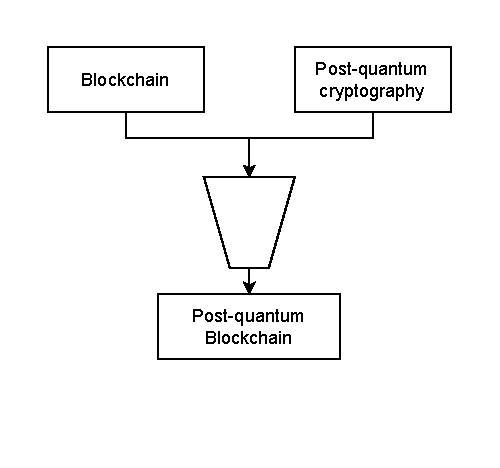
\includegraphics[width=22em]{img/mix.pdf}
\end{frame}

\begin{frame}
  \frametitle{Motivation}
  \centering
  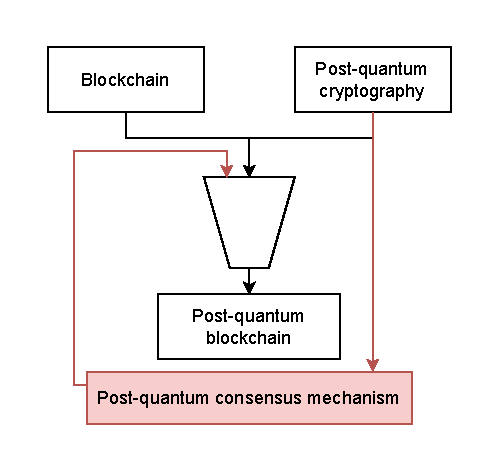
\includegraphics[width=22em]{img/mix-full.pdf}
\end{frame}


%%%%%%%%                       02 - Cíle práce                      %%%%%%%%
%---------------------------------------------------------------------------
% Stručně uveďte cíle Vaší práce.
% Vhodné jsou max. 3 odrážky/věty s hlavními cíli.

% Někdy je motivace totožná s formulací cílů. Nenuťte se do dvou slajdů, když je správnější myšlenku vyjádřit jedním... 

% Formulujte, co je cílem:
%  - Jak se pozná úspěšný výsledek?
%  - Co jsou výstupy?
%  - Jaké vlastnosti má mít úspěšný výsledek?
%  - Kde to půjde použít?

% Lepší je bez použití odrážek:
%  - mít dostatečně dobrý obrázek, který budete svými slovy komentovat 
%  - na obrázku je vizuální sdělení, sdělení slovní dodáte pusou

% Je zbytečné říkat generická a obecná tvrzení: "Řešení by mělo být rychlé, spolehlivé a robustní" - toto jsou obecné požadavky na cokoli a informační hodnota sdělení je NULA - je to jen plýtvání časem a inteligencí.
% Mluvte konkrétně: Jaké konkrétní vlastnosti má mít Vaše řešení, co konkrétně znamená "robustní", co konkrétně znamená "spolehlivé"?



% <<<<<<<<<<<<<<<<<<<<<<<<<<<<<<<<<<<<<<<<<<<<<<<<< %
% TU BUDE NIČ - povedané na predchádzajúcom snímku
% <<<<<<<<<<<<<<<<<<<<<<<<<<<<<<<<<<<<<<<<<<<<<<<<< %


\begin{frame}
  \frametitle{Objectives of the Thesis}
  \centering
  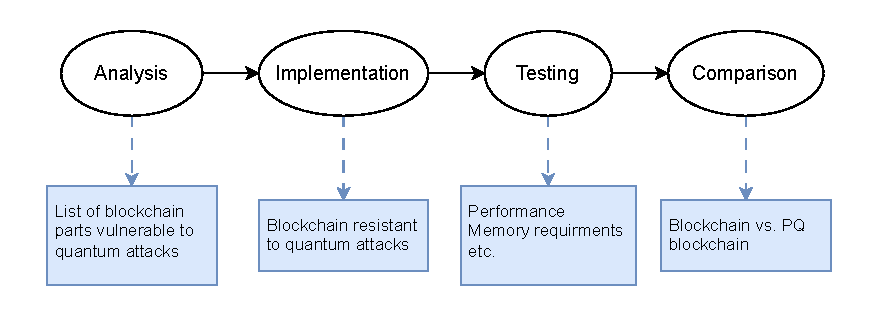
\includegraphics[width=\textwidth]{img/flow.pdf}
\end{frame}


%%%%%%%%                  03 - Informace o řešení                   %%%%%%%%
%---------------------------------------------------------------------------
% Cílem  obhajoby je podat zprávu o stavu projektu, nikoliv tedy držet přednášku na zadané téma. Mluvte o tom, co vy jste udělali, jaké jsou vaše výsledky. Mějte na slajdech formální pojmy, buďte přesní, definujte a odkazujte se.

% Prezentace nemusí a vlastně nemá obsahovat:
% -- Výklad použitých algoritmů apod. To patří do přednášky na dané téma, v prezentaci o stavu jen známé algoritmy uveďte podle jména, neznámé algoritmy třeba trochu přibližte, aby bylo zřejmo, o co jde, ale nevysvětlujte je podrobně. Není cílem, aby vaši posluchači algoritmu rozuměli a dokázali ho naprogramovat, ale aby měli představu, na čem pracujete a jak se vám to daří.
% -- Podrobnosti návrhu vašeho systému. Opět, posluchači nebudou váš systém hackovat, nepotřebují detailní strukturu tříd, názvy funkcí, jména souborů, datové formáty apod. Tyto věci uvádějte pouze v takové míře, která pomůže posluchačům udělat si představu, na čem pracujete a jak se vám to daří.

% HEROUT, Adam. Prezentování. Herout.net: Poznámky učitele, kouče, čtenáře. [online]. [cit. 2021-9-15]. Dostupné z: https://www.herout.net/blog/category/prezentovani/
%---------------------------------------------------------------------------

% - Uveďte, jaké zajímavé problémy jste v práci řešili.
% - Mělo by z toho být patrné, že je to závěrečná práce -- ne jen další projekt do předmětu -- tedy je v tom něco netriviálního, zajímavého a přínosného.
% - Raději dva nebo tři slajdy, které ukážete/vysvětlíte během 20 vteřin, než se snažit všechno "namastit" na jeden slajd.
% - Na slajdy je dobré dát vizuální informaci: vzorce, schemata, obrázky, diagramy. Slovní informaci můžete předat pusou. Je dokonale zbytečné a otravné mít na slajdu v odrážkách to samé, co se chystáte říct.
% - Titulek slajdu "Podstatné informace o řešení" je hodně generický. Ve skutečné Vaší prezentaci bude daleko lepší použít specifický titulek na každém ze slajdů, například: "Schéma neuronové sítě pro detekci frňáků", "Návrh nekonečného automatu", "Vytvořená datová sada" apod.


% <<<<<<<<<<<<<<<<<<<<<<<<<<<<<<<<<<<<<<<<<<<<<<<<< %
% 1. [Obr. 5.1] Návrh PQ blockchainu (high level view). Čo vlastne idem zabezpečovať? Aké sú hrozby? Čo som analyzoval? Aké algoritmy som vybral?

% Teraz ktým kritickým častiam blockchainu, ktoré som analyzoval ako zraniteľné voči kvantovým útokom a rozhodol som sa ich zabezpečiť. Chain of blockks, konsenzus mechanizmus, digitálne podpisy transakcií + šifrovanie BC komunikácie. Zo symetrickej kryptografie je dôležité používať hešovacie funkcie s dostatočným dĺžkov výstupu. Ja som sa rozhodol použiť SHA-512 aj keď podľa NÚKIB stačí SHA-386. Pre simetrické šifrovanie sa odporúča použiť dostatočne dlhý kľúč s 256+ bit odporúča sa AES-256. Asymetrickú kryptografiu môžeme rozdeliť na dva časti: digitálne podpisy a KEM. Tu je nutné použiť nové algoritmy práve zo súťaže NIST. Ja som sa rozhodol pre finalistov súťaže pre kategórie digitálnych podpisov sú to Falcon a Dilithium, SPHINCS+ je podľa mňa nepoužiteľný v blockchainoch, pre kategórie KEM som vybral jediný algoritmus pre ktorý výjde aj štandard a to algoritmus Kyber.

% 2. [Obr. 5.3] Implementácie. Ako vyzerá jeden node? Aké technológie som použil? Prečo som ich použil? Čo som abstrahoval (Moc sa tomu nevenovať. radšej hovoriť o tom čo som urobil ako neurobil.)? Popísať schému. Značný čas som strávil pri implementáciu P2P komunikácie. Zamerať sa na zaujímavosti a problémy, ktoré som riešil.

% Tento obrázok ukazuje komponenty jedného uzla a komunikáciu medzi týmito komponentami. Najväčšiu časť som strávil na tom ako vlastne pochopiť blockchain, keďže to pre mňa bola nová technológia a nevedel som akoby to malo správne fungovať. Koncept je jednoduchý, avšak praktická bola pre mňa celkom náročná. Najviac času som strávil hlavne pri vytváraní protokolu a P2P komunikácie. Storage je implementovaný ako LevelDB databáza, čo je embeded key value databáza a sú v nej uložené bloky, a účty (jedná sa o account base účet).

%  Abstrahoval som hlavne synchronizačné prvky...

% 3. Signer (veľmi krátko alebo možno ani nie)

% <<<<<<<<<<<<<<<<<<<<<<<<<<<<<<<<<<<<<<<<<<<<<<<<< %

\begin{frame}
    \frametitle{Vulnerable blockchain parts}
    \centering
    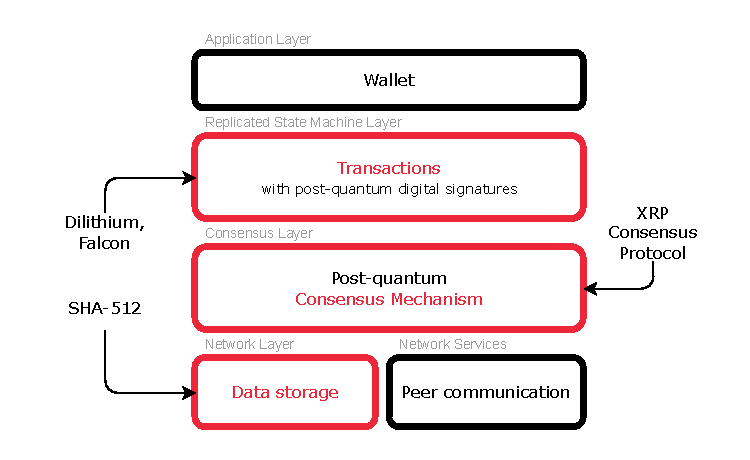
\includegraphics[width=34em]{img/bc-design-algs.pdf}
\end{frame}

\begin{frame}
    \frametitle{Node design}
    \centering
    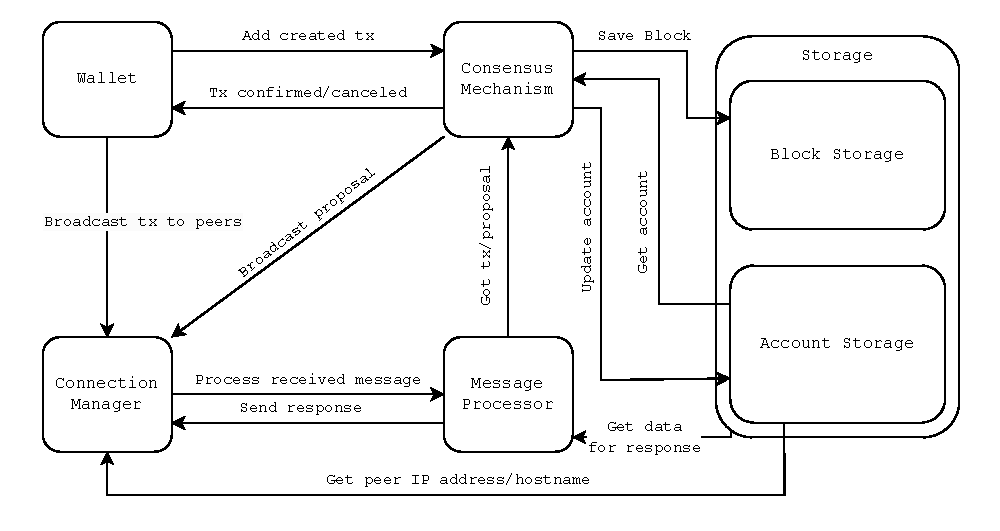
\includegraphics[width=\textwidth]{img/bc-design-pp.pdf}
\end{frame}

\begin{frame}
    \frametitle{Signer}
    \centering
    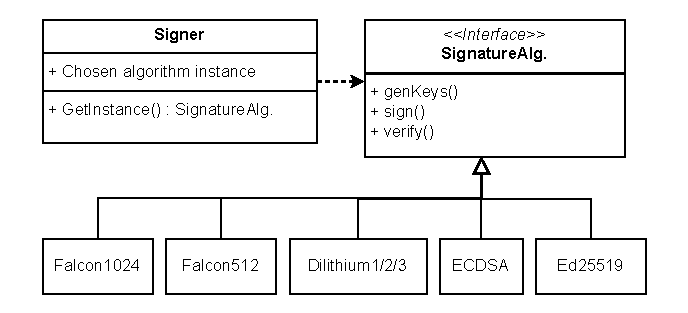
\includegraphics[width=\textwidth]{img/my-signer-ex.pdf}
\end{frame}


%%%%%%%%                    04 - Výsledky práce                     %%%%%%%%
%---------------------------------------------------------------------------
% Shrňte, jakých výsledků se Vám podařilo dosáhnout.
% Uveďte, jakým způsobem byla vyhodnocena funkčnost a správnost řešení.
% Buďte konkrétní: místo "Aplikace je otestovaná", řekněte, kým a jak byla testována, jaké byly výsledky testů.
% Místo "Úspěšnost detektoru je hodně dobrá" řekněte "Úspěšnost detektoru je 93 % mAP" nebo ještě radši ukažte tabulku se srovnáním oproti alternativním řešením.
% Pokud vyhodnocení sestávalo ze dvou nebo tří částí, může být vhodné rozdělit obsah na dva či tři slajdy. Při prezentování je ovšem potřeba se pohlídat, aby čas věnovaný každému slajdu byl adekvátně krátký a nedošlo k přetažení času.


% <<<<<<<<<<<<<<<<<<<<<<<<<<<<<<<<<<<<<<<<<<<<<<<<< %
% 1. [Obr. screen z testovanie/screeny] Čo som testoval? Ako som testoval?

% Testoval som algoritmy Falcon a Dilithium vo všetkých ich bezpečnostných úrovniach a porovnával som ich so súčasne používanými algoritmami ECDSA a Ed25519. Sledoval som 3 metriky. Množstvo procesorových cyklov, ktoré vykonal procesor pri jednotlivých algoritmoch, mnošstvo využitej pamäte (v jednom momente alokovanej programom) a mnošstvo dát, ktoré boli odoslané po sieti. Testovací scenár bol s 3, 5 10, 15 a 20 uzlami každý vytvoril v priebehu cca 50 sekúnd 20 transakcií. Všety získané výsledky sa priemerovali. Všetky uzly boli úplne prepojené 100% overlap.

% Testovanie prebiehalo automaticky pomocou vytvorených scriptov výsledky. Viď. obrázky. Pre testovanie som taktiež použil Docker. V každom kontaineri bežal jeden uzol.

% 2. Graf metrika cykly (výkon)

% Výkon zodpovedá bezpečnostným úrovniam daných algoritmov. Pročom z PQ algoritmov je nalepšie algoritmy falcon vďaka ich rýchlym overeniam podpisov, čo je najčastejšie využívaná funkcia v blockchainoch. Dilithium má rýchlejšie generovanie podpisov, ale Falcon vychádza stále lepšie. Dokonca je porovnateľný s algoritmom Ed25519. Samotný výkon PQ algoritmov je jeden z menších problémov pre PQ blockchainy. 

% 3. Graf metrika alokovaná pamäť

% Graf je viac sploštený, lebo som použil rýchly konsenzus mechanizmus a teda transackcie sa nekopia ale vzniká viac blokov častejšie čím rýchlejšie uvoľňuje alokovaná pamäť. Záver je, že rýchly konsenzus mechanizmus je výhodné použiť.

% 4. Graf množstvo prenesených dát

% Toto je pravdepodobne najväčší problém PQ kryptografie v blockchainoch. Veľkosti PQ podpisov a kľúčov je moc veľká. Problém je, že sa prenášaveľké mnošstvo dát s rastúcim počom transakcií sa to zhoršuje. Rastie náročnosť na množstvo prenášaných dát po sieti, ale aj celková veľkosť blockchainu.

% 5. Dôležité závery

% Hlavne analýza zraniteľných častí
% - Dostatočne silné hešovacie funkcie bez kolízií
% - PQ digitálne podpisy
% - Kvantovo odolný konsenzus mechnizmus
% - v okrajových prípadoch šifrovanie transakcií

% a závery testrovania
% - PQ algoritmy sú dostatočne rýchle
% - Výhodou je rýchly konsenzus mechanizmus
% - Najväščí problém je však veľkosť digitálnych podpisov a kľúčov a teda veľkosť samotného blockchainu a prenášaných dát.

% So svojím oponentom som sa rozprával a ukázal mi zaujímavé riešenie a tým je blockcahin Mina, ktorý má konštatntú veľkosť. Využíva zero-knowledge proofs.

% <<<<<<<<<<<<<<<<<<<<<<<<<<<<<<<<<<<<<<<<<<<<<<<<< %

%\begin{frame}
%    \frametitle{Test design}
%    \begin{columns}
%        \column{0.45\textwidth}
%        \begin{center}
%            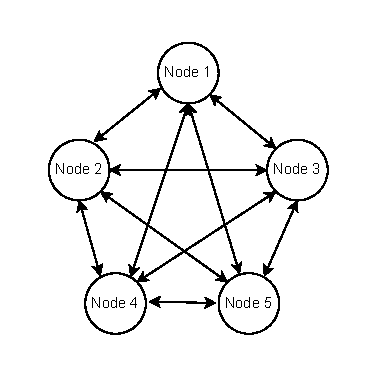
\includegraphics[width=20em]{img/nodes-net.pdf}
%        \end{center}
%        
%        \column{0.7\textwidth}
%        \begin{center}
%            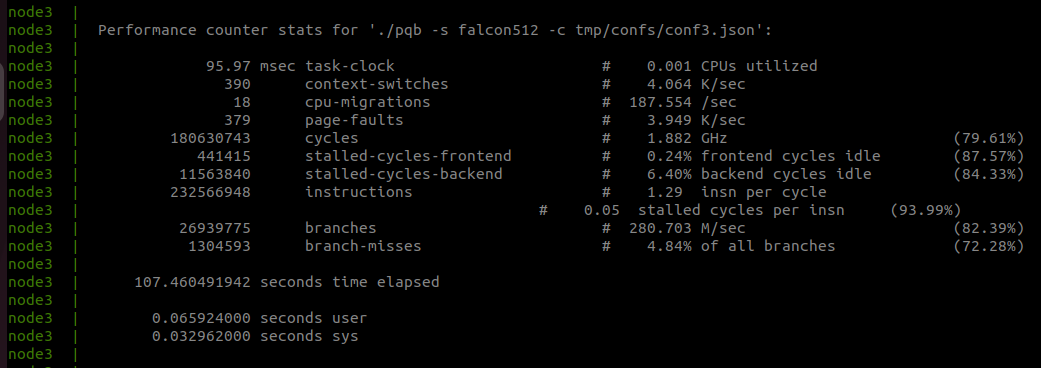
\includegraphics[width=25em]{img/node-stats.png}
%        \end{center}
%        \begin{itemize}
%            \item Performance
%            \item Memory requirments
%            \item Transferred data
%        \end{itemize}
%    \end{columns}
%\end{frame}


\begin{filecontents}{performance.dat}
Nodes	Falcon1024	Falcon512	Dilithium5	Dilithium3	Dilithium2	Ed25519	ECDSA
3	234676378	171252188	231943149	194608325	169059165	140671413	829826879
5	390314111	279384724	480440008	382570661	333922282	234052430	1454831824
10	1177845331	813948484	1762113322	1396466335	1146187859	676317939	4629475769
15	2247938023	1620714758	3385196110	3139504790	2513314458	1347373014	7556425358
20	3865946851	2845737681	5802784264	4759146393	4473290811	2287315562	11372690994
\end{filecontents}

\begin{frame}
    \frametitle{Performance}
    \begin{center}
    \begin{tikzpicture}
    \begin{axis}[
        grid=both,
        legend style={at={(0.5,-0.25)},anchor=north,legend columns=4,},
        width=\textwidth,
        height=6cm,
        xmin=0, xmax=25,
        xtick={3,5,10,15,20},
        xlabel={Number of nodes},
        ylabel={Processor cycles},
        xticklabels from table={performance.dat}{Nodes}
    ]
    
    \addplot[orange,smooth,mark=square*] table [y=Falcon1024,x=Nodes]{performance.dat};
    \addlegendentry{Falcon1024}
    
    \addplot[blue,smooth,mark=square*] table [y=Falcon512,x=Nodes]{performance.dat};
    \addlegendentry{Falcon512}
    
    \addplot[red,smooth,mark=square*] table [y=Dilithium5,x=Nodes]{performance.dat};
    \addlegendentry{Dilithium5}
    
    \addplot[violet,smooth,mark=square*] table [y=Dilithium3,x=Nodes]{performance.dat};
    \addlegendentry{Dilithium3}
    
    \addplot[cyan,smooth,mark=square*] table [y=Dilithium2,x=Nodes]{performance.dat};
    \addlegendentry{Dilithium2}
    
    \addplot[magenta,smooth,mark=square*] table [y=Ed25519,x=Nodes]{performance.dat};
    \addlegendentry{Ed25519}
    
    \addplot[brown,smooth,mark=square*] table [y=ECDSA,x=Nodes]{performance.dat};
    \addlegendentry{ECDSA}
        
    \end{axis}
    \end{tikzpicture}
    \end{center}
\end{frame}


\begin{filecontents}{memalloc.dat}
Nodes	Falcon1024	Falcon512	Dilithium5	Dilithium3	Dilithium2	Ed25519	ECDSA
3	4.448066667	4.353866667	4.810133333	4.584066667	4.426066667	4.127933333	4.2558
5	4.6016	4.40848	5.08852	4.82656	4.6028	4.1672	4.28816
10	4.89538	4.64106	5.67166	5.24632	4.9362	4.3062	4.43984
15	5.049786667	4.800733333	6.12876	5.5176	5.15992	4.412533333	4.5328
20	5.21861	4.92445	6.34903	5.8831	5.38804	4.55906	4.71704
\end{filecontents}

\begin{frame}
    \frametitle{Memory requirments}
    \begin{center}
    \begin{tikzpicture}
    \begin{axis}[
        grid=both,
        legend style={at={(0.5,-0.25)},anchor=north,legend columns=4,},
        width=\textwidth,
        height=6cm,
        xmin=0, xmax=25,
        xtick={3,5,10,15,20},
        xlabel={Number of nodes},
        ylabel={Allocated memory in MiB},
        xticklabels from table={memalloc.dat}{Nodes}
    ]
    
    \addplot[orange,smooth,mark=square*] table [y=Falcon1024,x=Nodes]{memalloc.dat};
    \addlegendentry{Falcon1024}
    
    \addplot[blue,smooth,mark=square*] table [y=Falcon512,x=Nodes]{memalloc.dat};
    \addlegendentry{Falcon512}
    
    \addplot[red,smooth,mark=square*] table [y=Dilithium5,x=Nodes]{memalloc.dat};
    \addlegendentry{Dilithium5}
    
    \addplot[violet,smooth,mark=square*] table [y=Dilithium3,x=Nodes]{memalloc.dat};
    \addlegendentry{Dilithium3}
    
    \addplot[cyan,smooth,mark=square*] table [y=Dilithium2,x=Nodes]{memalloc.dat};
    \addlegendentry{Dilithium2}
    
    \addplot[magenta,smooth,mark=square*] table [y=Ed25519,x=Nodes]{memalloc.dat};
    \addlegendentry{Ed25519}
    
    \addplot[brown,smooth,mark=square*] table [y=ECDSA,x=Nodes]{memalloc.dat};
    \addlegendentry{ECDSA}
        
    \end{axis}
    \end{tikzpicture}
    \end{center}
\end{frame}


\begin{filecontents}{transferred.dat}
Nodes	Falcon1024	Falcon512	Dilithium5	Dilithium3	Dilithium2	Ed25519	ECDSA
3	458815.7333	294589.3333	1556665.2	1146089.067	845482.4	101894.9333	103148.2667
5	1093492.36	687576.04	3946642.4	2606309.88	2156353.92	246896.96	235713.92
10	5273917.8	2867877.08	16473258.64	12048121.56	9021940.56	1012591.12	1023708.32
15	10714418.83	6183140.213	34401021.21	26922156.8	17976005.97	2199334.72	2070032.32
20	20232329.22	12265550.42	61978450.52	46281601.5	33881013.12	4340314.04	4106588.4
\end{filecontents}

\begin{frame}
    \frametitle{Transferred data}
    \begin{center}
    \begin{tikzpicture}
    \begin{axis}[
        grid=both,
        legend style={at={(0.5,-0.25)},anchor=north,legend columns=4,},
        width=\textwidth,
        height=6cm,
        xmin=0, xmax=25,
        xtick={3,5,10,15,20},
        xlabel={Number of nodes},
        ylabel={Amount of transferred data in bytes},
        xticklabels from table={transferred.dat}{Nodes}
    ]
    
    \addplot[orange,smooth,mark=square*] table [y=Falcon1024,x=Nodes]{transferred.dat};
    \addlegendentry{Falcon1024}
    
    \addplot[blue,smooth,mark=square*] table [y=Falcon512,x=Nodes]{transferred.dat};
    \addlegendentry{Falcon512}
    
    \addplot[red,smooth,mark=square*] table [y=Dilithium5,x=Nodes]{transferred.dat};
    \addlegendentry{Dilithium5}
    
    \addplot[violet,smooth,mark=square*] table [y=Dilithium3,x=Nodes]{transferred.dat};
    \addlegendentry{Dilithium3}
    
    \addplot[cyan,smooth,mark=square*] table [y=Dilithium2,x=Nodes]{transferred.dat};
    \addlegendentry{Dilithium2}
    
    \addplot[magenta,smooth,mark=square*] table [y=Ed25519,x=Nodes]{transferred.dat};
    \addlegendentry{Ed25519}
    
    \addplot[brown,smooth,mark=square*] table [y=ECDSA,x=Nodes]{transferred.dat};
    \addlegendentry{ECDSA}
        
    \end{axis}
    \end{tikzpicture}
    \end{center}
\end{frame}




%%%%%%%%                      05 - Poděkování                       %%%%%%%%
%---------------------------------------------------------------------------
% Na tomto slajdu by měl být buď jeden velký, nebo více menších vhodně poskládaných obrázků.
% Vyberte to nejlepší, čím se chcete pochlubit - komise se na tento slajd bude dívat nejdéle ze všech slajdů.
% U tohoto slajdu ústně poděkujete za pozornost (ne nutně textem přes celý slajd) a komise pak bude mít prostor pro jeho prohlížení při čtení posudků.
%---------------------------------------------------------------------------

% Co padne na konci prezentace, je to, co posluchači budou brát v úvahu při následném rozhodování.

% HEROUT, Adam. Prezentování. Herout.net: Poznámky učitele, kouče, čtenáře. [online]. [cit. 2021-9-15]. Dostupné z: https://www.herout.net/blog/category/prezentovani/
%---------------------------------------------------------------------------

\begin{frame}
    \frametitle{Thank You for Your Attention!}
    \centering
    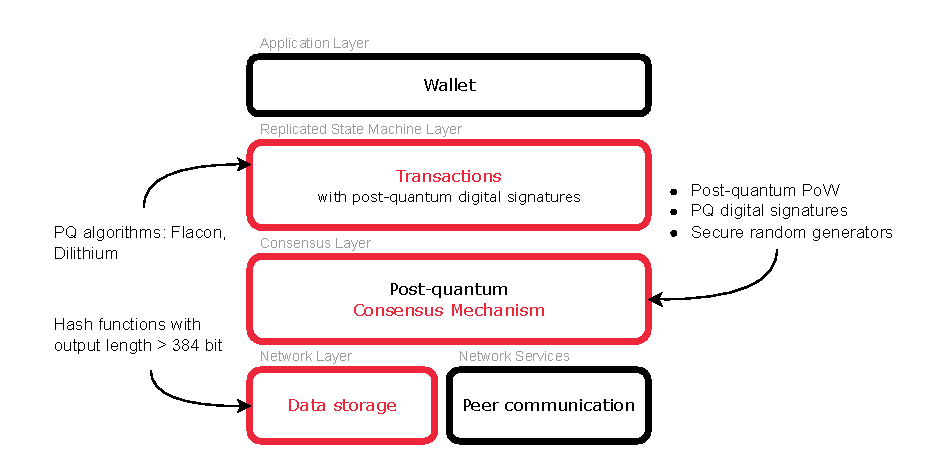
\includegraphics[width=\textwidth]{img/final.pdf}
\end{frame}


%%%%%%%%                        06 - Otázky                         %%%%%%%%
%---------------------------------------------------------------------------
% U státnic student:
%   1) Prezentuje o své práci, skončí "Děkuji za pozornost!"
%   2) Předseda komise organizuje, co bude dál: čte se výtah z posudků.
%   3) Student zodpoví otázky, které oponent napsal do svého posudku.
%   4) Student odpovídá na otázky, které padnou v místnosti: od členů komise, ale třeba i od hostů.

% Pro bod 3) výše je vhodné mít připravené slajdy, které v odpovídání pomůžou:
%   A) Ukážou doslovný text otázky oponenta, student ji přečte, aby ji všichni znali, a pak na ni odpoví.
%   B) Budou obsahovat vizuální pomůcky k odpovědi.
%       a) Některé odpovědi na otázky žádnou vizuální pomůcku nepotřebují: student prostě řekne odpověď a všechno je jasné.
%       b) U jiných odpovědí je rozumné mít připravený obrázek, tabulku, graf, cosi, na čem odpověď jasně ukáže.

% Otázky oponenta nebývají myšlené jako "témata na přednášku". Pokud je možné odpovědět jednou větou, je to lepší, než mlžit okolo.
% Vizuální pomůcky často pomáhají ke stručné odpovědi: "Na schématu je vidět, že problém X řeším takto." A hotovo...

% Pokud k otázkám nebude potřeba žádná vizuální informace, je vhodné mít jednotlivé otázky jako odrážky na jediném slajdu.
% Pokud je otázek více a jsou k nim obrázky či grafy, je vhodné mít pro každou otázku jeden slajd - nahoře znění otázky, pod ním vizuální materiál.

\appendix{}
\begin{frame}
    \frametitle{Opponent's Questions}
    Ako ovplyvňuje samotná implementácia postkvantových kryptografických algoritmov celkovú veľkosť~a účinnosť blockchainu? Ako by ste riešili potenciálne kompromisy~z hľadiska väčšej veľkosti~a väčších výpočtových požiadaviek~v akejkoľvek reálne nasadenej platforme blockchainu?
    
    \bigskip
    
    \begin{center}
        $\Sigma = B \times (H + C \times T)$
    \end{center}

    \begin{itemize}
        \item \emph{$\Sigma$}\,--\,celková veľkosť blockchainu
        \item \emph{B}\,--\,počet blokov
        \item \emph{H}\,--\,veľkosť hlavičky bloku
        \item \emph{C}\,--\,počet transackcii
        \item \emph{T}\,--\,veľkosť transakcie
    \end{itemize}
    
\end{frame}


\begin{frame}
    \frametitle{Opponent's Questions}
    Dajú sa postkvantové algoritmy použiť aj na generovanie distribuovanej náhodnosti, ktorá je dôležitá napr. v konsenzuálnych protokoloch Proof-of-Stake blockchainoch? Ako by ste to riešili? [1,2]; 1) ZKBdf: A ZKBoo-Based Quantum-Secure Verifiable Delay Function with Prover-Secret 2) Lattice-Based Proof-of-Work for Post-Quantum Blockchains

    \bigskip

    Účastníci blockchainu môžu spoločne prispievať k náhodnému výstupu vypočítaním VDF.

    \bigskip

    \emph{ZKBdf}

    \begin{itemize}
        \item Post-kvantovú odolnosť zaručuje nulová znalosť\,--\,kvantový počítač nedokáže predikovať výsledky VDF ostatných účastníkov blockchainu.
    \end{itemize}

    \emph{Lattice-Based Proof-of-Work}

    \begin{itemize}
        \item Post-kvantovú odolnosť zaručujú algoritmy založené na mriežkach.
    \end{itemize}
    
\end{frame}


\begin{frame}
    \frametitle{Key and ciphertext sizes (in bytes)\\for the KEM algorithms}
    \begin{table}[h]
    \centering
    \begin{tabular}[p]{| c | c | c | c | c |}
        \hline
        \textbf{Algorithm} & \textbf{Claimed Security} & \textbf{Public key} & \textbf{Private key} & \textbf{Ciphertext} \\ \hline
        \textsc{Kyber512} & Level 1 & 800 & 1632 & 768 \\
        \textsc{Kyber768} & Level 3 & 1\,184 & 2\,400 & 1\,088 \\
        \textsc{Kyber1024} & Level 5 & 1\,568 & 3\,168 & 1\,568 \\
        \hline
        Classic McEliece348864 & Level 1 &  261\,120 & 6\,492 & 128 \\
        Classic McEliece460896 & Level 3 & 524\,160 & 13\,608 & 188 \\
        Classic McEliece6688128 & Level 5 & 104\,992 & 13\,932 & 240 \\
        Classic McEliece6960119 & Level 5 & 1\,047 319 & 13\,948 & 226 \\
        Classic McEliece8192128 & Level 5 & 1\,357 824 & 14\,120 & 240 \\
        \hline
        HQC-128 & Level 1 & 2\,249 & 40 & 4\,481 \\
        HQC-192 & Level 3 & 4\,522 & 40 & 9\,026 \\
        HQC-256 & Level 5 & 7\,245 & 40 & 14\,469 \\
        \hline
    \end{tabular}
    \end{table}
\end{frame}


\begin{frame}
    \frametitle{Key and signature sizes (in bytes)\\for the digital signatures algorithms}
    \begin{table}[h]
    \centering
    \begin{tabular}[p]{| c | c | c | c | c |}
        \hline
        \textbf{Algorithm} & \textbf{Claimed Security} & \textbf{Public key} & \textbf{Private key} & \textbf{Signature} \\ \hline
        \multirow{3}{*}{Dilithium} & Level 2 & 1\,312 & 2\,528 & 2\,420 \\
        & Level 3 & 1\,952 & 4\,000 & 3\,293 \\
        & Level 5 & 2\,592 & 4\,864 & 4\,595 \\
        \hline
        \textsc{Falcon}-512 & Level 1 & 897 & 7\,553 & 666 \\
        \textsc{Falcon}-1024 & Level 5 & 1\,793 & 13\,953 & 1\,280 \\
        \hline
        SPHINCS$^+$-128s & Level 1 & 32 & 64 & 7\,856 \\
        SPHINCS$^+$-128f & Level 1 & 32 & 64 & 17\,088 \\
        SPHINCS$^+$-192s & Level 3 & 48 & 96 & 16\,224 \\
        SPHINCS$^+$-192f & Level 3 & 48 & 96 & 35\,664 \\
        SPHINCS$^+$-256s & Level 5 & 64 & 128 & 29\,792 \\
        SPHINCS$^+$-256f & Level 5 & 64 & 128 & 49\,856 \\
        \hline
    \end{tabular}
    \end{table}
\end{frame}

\begin{frame}
    \frametitle{Performance of KEM algorithms\\(in processor cycles)}
    \begin{table}[h]
    \centering
    \begin{tabular}[p]{| c | c | c | c | c |}
        \hline
        \textbf{Algorithm} & \textbf{Keygen} & \textbf{Encapsulation} & \textbf{Decapsulation} \\ \hline
        \textsc{Kyber512} & 29\,172 & 36\,768 & 26\,943 \\
        \textsc{Kyber768} & 45\,407 & 54\,332 & 42\,098 \\
        \textsc{Kyber1024} & 61\,960 & 74\,939 & 60\,053 \\
        \hline
        Classic McEliece348864 & 151\,761\,145 & 47\,503 & 119\,873 \\
        Classic McEliece460896 & 385\,383\,414 & 90\,694 & 231\,764 \\
        Classic McEliece6688128 & 591\,004\,800 & 191\,851 & 273\,034 \\
        Classic McEliece6960119 & 567\,788\,742 & 164\,539 & 251\,788 \\
        Classic McEliece8192128 & 625\,667\,532 & 203\,624 & 268\,867 \\
        \hline
        HQC-128 & 104\,115 & 197\,030 & 360\,575 \\
        HQC-192 & 244\,636 & 459\,309 & 766\,797 \\
        HQC-256 & 447\,179 & 845\,083 & 1\,425\,978 \\
        \hline
    \end{tabular}
    \end{table}
\end{frame}


\begin{frame}
    \frametitle{Performance of signature algorithms\\(in processor cycles)}
    \begin{table}[h]
    \centering
    \begin{tabular}[p]{| c | c | c | c | c |}
        \hline
        \textbf{Algorithm} & \textbf{Keygen} & \textbf{Signing} & \textbf{Verifycation}\\ \hline
        Dilithium2 & 90\,195 & 236\,975 & 87\,348 \\
        Dilithium3 & 153\,215 & 380\,755 & 144\,980 \\
        Dilithium5 & 247\,152 & 476\,989 & 236\,726 \\
        \hline
        \textsc{Falcon}-512 & 21\,234\,790 & 888\,844 & 143\,976 \\
        \textsc{Falcon}-1024 & 63\,158\,867 & 1\,800\,943 & 292\,065 \\
        \hline
        SPHINCS$^+$-128s & 5\,9910\,564 & 447\,597\,974 & 745\,416 \\
        SPHINCS$^+$-128f & 933\,692 & 21\,966\,943 & 1\,891\,461 \\
        SPHINCS$^+$-192s & 96\,144\,674 & 1\,080\,729\,340 & 1\,152\,859 \\
        SPHINCS$^+$-192f & 1\,405\,335 & 38\,270\,621 & 2\,709\,479 \\
        SPHINCS$^+$-256s & 59\,723\,455 & 786\,789\,398 & 1\,565\,715 \\
        SPHINCS$^+$-256f & 3\,740\,593 & 79\,046\,495 & 2\,729\,293 \\
        \hline
    \end{tabular}
    \end{table}
\end{frame}

  % Slajdy v angličtině / Slides in English
    \fi
\end{document}

%---------------------------------------------------------------------------
% Když připravujete prezentaci, rozmyslete, co budete říkat, pak rozmyslete, co by se k tomu hodilo mít promítnuté na plátně za vámi a pak podle toho připravte slajdy.

% Co je špatného na slajdech s mnoha písmenky
% -- Jejich nejčastější problém bývá, že slajd sděluje řečníkovu myšlenku. Po zobrazení slajdu si ho během několika vteřin všichni přečtou (a – chcete-li – během této doby řečníka neposlouchají). Potom řečník svoje publikum k smrti nudí tím, že jim říká, co už vědí – co se dočetli na slajdu.
% -- Stejné chyby se dopustí i ten, kdo svoji pointu sdělí stručným slajdem o čtyřech slovech, i ten, kdo svoji pointu proflákne roztomilým nákresíčkem.
% -- Slajd musí být hádanka – když se zobrazí, posluchač mu ještě moc nerozumí, neví, proč tu je. Pak, jak řečník mluví a vysvětluje, slajd dává víc a víc smysl, až dojde k prozření: „AHA, jasně!“

% Pár námětů na zamyšlení nad hotovými slajdy:
% -- Jsem se slajdy spokojený? S čím nejvíc, s čím nejmíň?
% -- Od kterých jednotlivých slajdů čekám, že posluchače nadchnou, nakloní na mou stranu?
% -- Kdyby mi někdo chtěl pokládat nepříjemné otázky – do kterého slajdu se bude strefovat?
% -- Které slajdy budou samy o sobě přitahovat pozornost posluchačů jen se objeví? Které slajdy budou nudit a budu pozornost ztrácet?
% -- Jaký „první dojem“ o vás sdělují první tři slajdy? „Tento student je …“ – co si komise doplní místo třech teček?



% HEROUT, Adam. Prezentování. Herout.net: Poznámky učitele, kouče, čtenáře. [online]. [cit. 2021-9-15]. Dostupné z: https://www.herout.net/blog/category/prezentovani/
%---------------------------------------------------------------------------
